\documentclass{beamer}
\usepackage{../../shared/styles/custom}
% =============================================================================
% ML TEACHING MATHEMATICAL NOTATION CONVENTIONS
% =============================================================================
% Based on standard ML textbooks: Murphy's "Machine Learning: A Probabilistic Perspective",
% Bishop's "Pattern Recognition and Machine Learning", and "Mathematics for Machine Learning"

% =============================================================================
% CORE NOTATION STANDARDS
% =============================================================================

% SCALARS: Regular italics (lowercase for variables, uppercase for constants)
% Examples: x, y, n, d, k, \theta, \alpha, \lambda, \sigma

% VECTORS: Bold lowercase letters
% Examples: \mathbf{x}, \mathbf{w}, \mathbf{\mu}, \mathbf{\theta}

% MATRICES: Bold uppercase letters
% Examples: \mathbf{X}, \mathbf{W}, \mathbf{\Sigma}, \mathbf{\Lambda}

% SETS: Calligraphic uppercase
% Examples: \mathcal{D}, \mathcal{X}, \mathcal{Y}

% SPACES: Blackboard bold
% Examples: \mathbb{R}, \mathbb{Z}, \mathbb{N}

% =============================================================================
% VECTOR NOTATION (bold lowercase)
% =============================================================================

\newcommand{\vx}{\mathbf{x}}        % Input vector
\newcommand{\vy}{\mathbf{y}}        % Output vector
\newcommand{\vw}{\mathbf{w}}        % Weight vector
\newcommand{\vb}{\mathbf{b}}        % Bias vector
\newcommand{\vh}{\mathbf{h}}        % Hidden vector
\newcommand{\vz}{\mathbf{z}}        % Latent vector
\newcommand{\vf}{\mathbf{f}}        % Function vector
\newcommand{\vg}{\mathbf{g}}        % Gradient vector
\newcommand{\vu}{\mathbf{u}}        % Generic vector u
\newcommand{\vv}{\mathbf{v}}        % Generic vector v
\newcommand{\vzero}{\mathbf{0}}     % Zero vector
\newcommand{\vone}{\mathbf{1}}      % Ones vector

% Greek vectors (bold)
\newcommand{\vmu}{\boldsymbol{\mu}}     % Mean vector
\newcommand{\vtheta}{\boldsymbol{\theta}} % Parameter vector
\newcommand{\vlambda}{\boldsymbol{\lambda}} % Lambda vector
\newcommand{\valpha}{\boldsymbol{\alpha}}   % Alpha vector
\newcommand{\vbeta}{\boldsymbol{\beta}}     % Beta vector
\newcommand{\vxi}{\boldsymbol{\xi}}         % Xi vector
\newcommand{\vepsilon}{\boldsymbol{\epsilon}} % Epsilon vector

% =============================================================================
% MATRIX NOTATION (bold uppercase)
% =============================================================================

\newcommand{\mX}{\mathbf{X}}        % Data matrix
\newcommand{\mY}{\mathbf{Y}}        % Target matrix
\newcommand{\mW}{\mathbf{W}}        % Weight matrix
\newcommand{\mA}{\mathbf{A}}        % Generic matrix A
\newcommand{\mB}{\mathbf{B}}        % Generic matrix B
\newcommand{\mC}{\mathbf{C}}        % Generic matrix C
\newcommand{\mH}{\mathbf{H}}        % Hidden layer matrix / Hessian
\newcommand{\mI}{\mathbf{I}}        % Identity matrix
\newcommand{\mJ}{\mathbf{J}}        % Jacobian matrix
\newcommand{\mK}{\mathbf{K}}        % Kernel matrix
\newcommand{\mL}{\mathbf{L}}        % Loss matrix / Cholesky factor
\newcommand{\mP}{\mathbf{P}}        % Projection matrix
\newcommand{\mQ}{\mathbf{Q}}        % Orthogonal matrix
\newcommand{\mR}{\mathbf{R}}        % Rotation matrix
\newcommand{\mS}{\mathbf{S}}        % Scatter matrix
\newcommand{\mU}{\mathbf{U}}        % Left singular vectors
\newcommand{\mV}{\mathbf{V}}        % Right singular vectors

% Greek matrices (bold)
\newcommand{\mSigma}{\boldsymbol{\Sigma}}   % Covariance matrix
\newcommand{\mLambda}{\boldsymbol{\Lambda}} % Diagonal eigenvalue matrix
\newcommand{\mPhi}{\boldsymbol{\Phi}}       % Feature matrix
\newcommand{\mPsi}{\boldsymbol{\Psi}}       % Basis matrix
\newcommand{\mTheta}{\boldsymbol{\Theta}}   % Parameter matrix

% =============================================================================
% SETS AND SPACES (following Bishop/Murphy conventions)
% =============================================================================

\newcommand{\cD}{\mathcal{D}}       % Dataset
\newcommand{\cH}{\mathcal{H}}       % Hypothesis space
\newcommand{\cX}{\mathcal{X}}       % Input space
\newcommand{\cY}{\mathcal{Y}}       % Output space
\newcommand{\cF}{\mathcal{F}}       % Function space
\newcommand{\cG}{\mathcal{G}}       % Gaussian process
\newcommand{\cL}{\mathcal{L}}       % Lagrangian / Loss
\newcommand{\cN}{\mathcal{N}}       % Normal distribution
\newcommand{\cU}{\mathcal{U}}       % Uniform distribution
\newcommand{\cB}{\mathcal{B}}       % Bernoulli distribution
\newcommand{\cP}{\mathcal{P}}       % Probability distribution

% Number systems
\newcommand{\Real}{\mathbb{R}}      % Real numbers
\newcommand{\Nat}{\mathbb{N}}       % Natural numbers
\newcommand{\Int}{\mathbb{Z}}       % Integers
\newcommand{\Complex}{\mathbb{C}}   % Complex numbers

% =============================================================================
% OPERATORS AND FUNCTIONS (following standard conventions)
% =============================================================================

% Prediction notation (commonly used in ML)
\newcommand{\yhat}{\hat{\vy}}        % Predicted output vector (bold)
\newcommand{\yhati}{\hat{y}_i}       % Predicted output for sample i (scalar)

% Common ML functions (with conflict resolution)
\providecommand{\sigmoid}{}
\renewcommand{\sigmoid}{\operatorname{sigmoid}}
\providecommand{\softmax}{}
\renewcommand{\softmax}{\operatorname{softmax}}
\providecommand{\ReLU}{}
\renewcommand{\ReLU}{\operatorname{ReLU}}
\providecommand{\sign}{}
\renewcommand{\sign}{\operatorname{sign}}
\DeclareMathOperator{\Gain}{Gain}    % Information gain
\DeclareMathOperator{\Entropy}{Entropy}
% KL divergence (check for conflicts)
\providecommand{\KL}{}
\renewcommand{\KL}{\operatorname{KL}}
\DeclareMathOperator{\MSE}{MSE}      % Mean squared error
\DeclareMathOperator{\MAE}{MAE}      % Mean absolute error
\DeclareMathOperator{\RMSE}{RMSE}    % Root mean squared error

% Classification metrics (upright text)
\newcommand{\TP}{\text{TP}}          % True positives
\newcommand{\TN}{\text{TN}}          % True negatives  
\newcommand{\FP}{\text{FP}}          % False positives
\newcommand{\FN}{\text{FN}}          % False negatives
\DeclareMathOperator{\Precision}{Precision}
\DeclareMathOperator{\Recall}{Recall}
\DeclareMathOperator{\Accuracy}{Accuracy}

% Transpose and inverse
\newcommand{\tp}{^\top}             % Transpose (Bishop/Murphy style)
\newcommand{\inv}{^{-1}}            % Matrix inverse
\newcommand{\pinv}{^{\dagger}}      % Pseudoinverse

% Norms (consistent with Murphy/Bishop)
\newcommand{\norm}[1]{\|#1\|}       % Generic norm
\newcommand{\normone}[1]{\|#1\|_1}  % L1 norm
\newcommand{\normtwo}[1]{\|#1\|_2}  % L2 norm
\newcommand{\norminf}[1]{\|#1\|_\infty} % L-infinity norm
\newcommand{\normF}[1]{\|#1\|_F}    % Frobenius norm

% Optimization operators (upright as in Murphy)
\providecommand{\argmin}{}
\renewcommand{\argmin}{\operatorname*{arg\,min}}
\providecommand{\argmax}{}
\renewcommand{\argmax}{\operatorname*{arg\,max}}
\DeclareMathOperator{\minimize}{minimize}
\DeclareMathOperator{\maximize}{maximize}
\DeclareMathOperator{\subjectto}{subject\,to}

% Matrix operations (upright) - use conditional definitions
\providecommand{\tr}{}
\renewcommand{\tr}{\operatorname{tr}}       % Trace
\providecommand{\det}{}
\renewcommand{\det}{\operatorname{det}}     % Determinant
\providecommand{\rank}{}
\renewcommand{\rank}{\operatorname{rank}}   % Rank
\providecommand{\span}{}
\renewcommand{\span}{\operatorname{span}}   % Span
\providecommand{\null}{}
\renewcommand{\null}{\operatorname{null}}   % Null space
\DeclareMathOperator{\range}{range} % Range/column space
\providecommand{\diag}{}
\renewcommand{\diag}{\operatorname{diag}}   % Diagonal operator
\providecommand{\vec}{}
\renewcommand{\vec}{\operatorname{vec}}     % Vectorization operator

% Probability and statistics (Murphy/Bishop style)
\newcommand{\Prob}{\mathbb{P}}      % Probability measure
\newcommand{\Exp}{\mathbb{E}}       % Expectation
\DeclareMathOperator{\Var}{Var}     % Variance
\DeclareMathOperator{\Cov}{Cov}     % Covariance
\DeclareMathOperator{\Corr}{Corr}   % Correlation
% KL divergence already defined above
\DeclareMathOperator{\MI}{I}        % Mutual information

% Activation functions (already defined above with conflict resolution)

% =============================================================================
% STANDARD PARAMETER CONVENTIONS (Murphy/Bishop style)
% =============================================================================

% Primary parameters: θ (theta) - following Murphy's convention
% Learning rates: α, η (alpha, eta)
% Regularization: λ (lambda)
% Precision: β (beta) - following Bishop
% Variance: σ² (sigma squared)
% Standard deviation: σ (sigma)
% Mean: μ (mu)

% Common scalars:
% n - number of training examples
% d - dimensionality of input
% k - number of classes/clusters
% m - number of hidden units
% T - number of time steps
% i, j - indices

% =============================================================================
% STANDARD NOTATION EXAMPLES (Murphy/Bishop style)
% =============================================================================

% Linear regression:      y = \vw\tp\vx + b
% Matrix form:            \vy = \mX\vw + b\vone
% Logistic regression:    p(y=1|\vx) = \sigmoid(\vw\tp\vx)
% Gaussian:               \vx \sim \cN(\vmu, \mSigma)
% Parameter update:       \vtheta_{t+1} = \vtheta_t - \alpha \nabla \cL(\vtheta_t)
% Likelihood:             p(\cD|\vtheta) = \prod_{i=1}^n p(y_i|\vx_i, \vtheta)
% Posterior:              p(\vtheta|\cD) \propto p(\cD|\vtheta)p(\vtheta)
% Prediction:             p(y^*|\vx^*, \cD) = \int p(y^*|\vx^*, \vtheta)p(\vtheta|\cD)d\vtheta

% =============================================================================
% COMMON MISTAKES TO AVOID
% =============================================================================

% ❌ WRONG NOTATION          →  ✅ CORRECT NOTATION (Murphy/Bishop style)

% Transpose:
% ❌ x^t, X^t              →  ✅ \vx\tp, \mX\tp
% ❌ x', X'                →  ✅ \vx\tp, \mX\tp

% Vectors vs Matrices vs Scalars:
% ❌ X (for vector)        →  ✅ \vx (bold lowercase)
% ❌ w (for weight vector) →  ✅ \vw (bold lowercase)
% ❌ x (for data matrix)   →  ✅ \mX (bold uppercase)
% ❌ \mathbf{\theta}       →  ✅ \vtheta (Greek vectors are bold)
% ❌ \mathbf{n}            →  ✅ n (scalars are not bold)

% Sets and distributions:
% ❌ R                     →  ✅ \Real (blackboard bold for number systems)
% ❌ \mathcal{R}           →  ✅ \Real (use blackboard for reals)
% ❌ Normal               →  ✅ \cN (calligraphic for distributions)

% Functions and operators:
% ❌ argmax                →  ✅ \argmax (upright operator)
% ❌ E[X]                  →  ✅ \Exp[X] (blackboard E for expectation)
% ❌ trace(A)              →  ✅ \tr(\mA) (upright operator)

% =============================================================================
% ALGORITHM NAME CONVENTIONS
% =============================================================================

% Use standard capitalizations as in textbooks:
% k-NN, SVM, PCA, GMM, EM, MAP, ML, SGD, Adam, RMSprop
% ReLU, tanh, sigmoid, softmax

\endinput



\newcommand{\vecuvec}[2] %start point, end point (of vector)
{   \VECTORSUB(#2)(#1)(\sola,\solb,\solc)
	\UNITVECTOR(\sola, \solb, \solc)(\sola,\solb,\solc)
	%arrow in blue
	\draw[->,thick,blue] (#1) -- (#2); 
	%corresponding unit-vector in red:
	\edef\temp{\noexpand\draw[->, thick,red] (#1) -- ($(#1)+(\sola,\solb,\solc)$);}
	\temp
}


%\beamerdefaultoverlayspecification{<+->}






\title{Linear Regression}
\date{\today}
\author{Nipun Batra and the teaching staff}
\institute{IIT Gandhinagar}
\begin{document}
  \maketitle
  

\section{Setup}
  
% \section{Linear Regression}

\begin{frame}{Linear Regression}
\begin{itemize}
	
	
	\item<+-> Output is continuous in nature.
	\item<+-> Examples of linear systems:
	\begin{itemize}
		\item<+-> $F=ma$
		\item<+-> $v=u+at$
	\end{itemize}
	
\end{itemize}
\end{frame}

\begin{frame}{Task at hand}
\begin{itemize}

\item TASK: Predict Weight = f(height)
\end{itemize}
\begin{center}
    

\begin{tabular}{ |c|c|c|c| } 
\hline
 Height & Weight \\
\hline
3 & 29 \\ 
4 & 35 \\ 
5 & 39\\
2 & 20\\
6 & 41\\
\hline
\hline
7 & ?\\
8 & ?\\
1 &? \\
\hline
\end{tabular}

\end{center}
The first part of the dataset is the training points. The latter ones are testing points.	

\end{frame}


\begin{frame}{Scatter Plot}
\begin{tikzpicture}

\pgfplotsset{
	scale only axis,
}

\begin{axis}[
xlabel=$height~(ft)$,
ylabel=$weight~(kg)$,
xmin=0,
axis x line*=bottom,
axis y line*=left,
xtick align=outside,
ytick align=outside
]

\addplot[only marks, mark=*]
coordinates{ % plot 1 data set
	(6, 80)
	(5.5, 80)
	(6, 70)
	(5, 40)
	(5, 60)
	(4, 30)
	(4, 45)
	(4, 20)
	(6, 120)
	(2, 15)
	(1, 5)
	(0.5, 4)
	(3, 20)
	(6, 62)
	(5, 57)
	

	% more points...
}; 
\node[label={180:{Outlier}},circle,fill,inner sep=2pt] at (axis cs:6,120) {};
\node[label={-90:{Outlier}},circle,fill,inner sep=2pt] at (axis cs:4,20) {};

% plot 1 legend entry


\end{axis}

\end{tikzpicture}


\end{frame}


\begin{frame}{Matrix representation of the expression}


\begin{itemize}
\item $weight_{1} \approx \theta_{0} + \theta_{1} \cdot height_{1}$

\item $weight_{2} \approx \theta_{0} + \theta_{1} \cdot height_{2}$

\item $weight_{N} \approx \theta_{0} + \theta_{1} \cdot height_{N}$

\end{itemize}
\begin{center}
\pause	\begin{tcolorbox}
		$weight_{i} \approx \theta_{0} + \theta_{1} \cdot height_{i}$
	\end{tcolorbox}
\end{center}
\end{frame}



\begin{frame}{Matrix representation of the expression}



\[\begin{bmatrix}
    weight_{1}   \\
    weight_{2}   \\
    \dots \\
    weight_{N}
\end{bmatrix}
= \begin{bmatrix}
    1& height_{1}   \\
    1& height_{2}   \\
    \dots & \dots  \\
    1& height_{N}   \\
\end{bmatrix}
\begin{bmatrix}
    \theta_{0} \\
    \theta_{1}
\end{bmatrix}\] \\

\pause \[\yhat_{n \times 1} = \mX_{n \times d} \vtheta_{d \times 1} \]


%W(N \times 1); X(N\times 2); \theta(2 \times 1);


\pause \begin{itemize}
    \item<+-> $\theta_{0}$ - Bias Term/Intercept Term
    \item<+-> $\theta_{1}$ - Slope
\end{itemize}
\end{frame}



\begin{frame}{Extension to multiple dimensions}

In the previous example y = f(x), where x is one-dimensional.\\
\pause Examples in multiple dimensions.\\
\pause One example is to predict the water demand of the IITGN campus

\small{
\begin{center}
  \pause  \begin{tcolorbox}
        Demand = f(\# occupants, Temperature)
    \end{tcolorbox}
\end{center}

\begin{center}
    \pause \begin{tcolorbox}
        Demand = Base Demand + $K_{1}$ * \# occupants + $K_{2}$ * Temperature
    \end{tcolorbox}
\end{center}
}

\end{frame}

\begin{frame}{Intuition}
    We hope to: 
    \begin{itemize}
        \item Learn $f$: $Demand$ = $f(\# occupants, Temperature)$
        \item From training dataset
        \item To predict the condition for the testing set
    \end{itemize}
\end{frame}


\begin{frame}{Linear Relationship}
    We have 
    \begin{itemize}[<+->]
    	\item $x_i = \begin{bmatrix}
    	Temperature_i\\\#Occupants_i
    	\end{bmatrix}$
        \item Estimated demand for $i^{th}$ sample is  $\hat{demand_{i}} = \theta_{0} + \theta_{1} Temperature_i + \theta_{2} Occupants_i$
        \item $\hat{demand_{i}} = x_{i}'^{T} \theta$
        \item where $\theta = \begin{bmatrix}\theta_0\\\theta_1\\ \theta_2
        \end{bmatrix}$
        \item and $x_{i}' = \begin{bmatrix}
        1\\Temperature_i\\\#Occupants_i
        \end{bmatrix} = \begin{bmatrix}
        1 \\ x_i
        \end{bmatrix}$
        \item Notice the transpose in the equation! This is because $x_{i}$ is a column vector
    \end{itemize}

\end{frame}





\begin{frame}{We can expect the following}
    \begin{itemize}
        \item<+-> Demand increases, if \# occupants increases, then $\theta_{2}$ is likely to be positive
        
        \item<+-> Demand increases, if temperature increases, then $\theta_{1}$ is likely to be positive
        
        \item<+-> Base demand is independent of the temperature and the \# occupants, but, likely positive, thus $\theta_0$ is likely positive.
        
    \end{itemize}
\end{frame}


\section{Normal Equation}
\begin{frame}{Generalized Linear Regression Format}
\begin{itemize}[<+->]
	\item Assuming $N$ samples for training
	\item \# Features = $M$
\end{itemize}


   \pause \[\begin{bmatrix}
        \hat{y_{1}}\\
        \hat{y_{2}} \\
        \vdots \\
        \hat{y_{N}}
    \end{bmatrix}_{N \times 1}
    =     \begin{bmatrix}
        1 & x_{1,1} & x_{1,2} & \dots & x_{1,M}\\
        1 & x_{2,1} & x_{2,2} & \dots & x_{2,M}\\
        \vdots & \vdots & \vdots & \dots & \vdots\\
        1 & x_{N,1} & x_{N,2} & \dots & x_{N,M}\\
        % y_{2} \\
        % \vdots \\
        % y_{N}
    \end{bmatrix}_{N \times (M+1)}
    \begin{bmatrix}
        \theta_{0}\\
        \theta_{1}\\
        \vdots \\
        \theta_{M}\\
    \end{bmatrix}_{(M+1)\times 1}
   \]
   
%   \begin{center}
%       \textbf{Y}: N\times1; \textbf{X}: N\times(M+1); $\mathbf{\theta}$: (M+1)\times1 
%   \end{center}
   
  \pause  \begin{tcolorbox}
   \begin{center}
       
   

   $ \hat{Y} = X\theta$
   \end{center}
   \end{tcolorbox}

   
\end{frame}


\begin{frame}{Relationships between feature and target variables}
    \begin{itemize}
    	\item  There could be different $\theta_{0}, \theta_{1} \dots \theta_{M}$. Each of them can represents a relationship.
    	\item  Given multiples values of $\theta_{0}, \theta_{1} \dots \theta_{M}$ how to choose which is the  best?
    	\item Let us consider an example in 2d
    \end{itemize}
   
    
   
    
\end{frame}

\begin{frame}{Relationships between feature and target variables}
Out of the three fits, which one do we choose? \vspace{10pt}
\begin{tikzpicture}

\pgfplotsset{
	scale only axis,
}

\begin{axis}[
xlabel=$x$,
ylabel=$y$,
xmin=-1,
axis x line*=bottom,
axis y line*=left,
xtick align=outside,
ytick align=outside,
legend pos=outer north east
]

\addplot[mark=none,blue] {x};\addlegendentry{$\hat{y}=0+1x$}
\addplot[mark=none,yellow] {x+2};\addlegendentry{$\hat{y}=2+1x$}
\addplot[mark=none,green] {2*x-2};\addlegendentry{$\hat{y}=-2+2x$}
\addplot[only marks, mark=*]
coordinates{ % plot 1 data set
	(0,0)
	(1,1)
	(2,2)
	(3,3)
	% more points...
}; \addlegendentry{Train data}


% plot 1 legend entry


\end{axis}

\end{tikzpicture}

\end{frame}


\begin{frame}{Relationships between feature and target variables}
We have $\hat{y}=2+1x$ as one relationship.\vspace{10pt}
\begin{tikzpicture}

\pgfplotsset{
	scale only axis,
}

\begin{axis}[
xlabel=$x$,
ylabel=$y$,
xmin=-1,
axis x line*=bottom,
axis y line*=left,
xtick align=outside,
ytick align=outside,
legend pos=outer north east
]


\addplot[mark=none,yellow] {x+2};\addlegendentry{$\hat{y}=2+1x$}
\addplot[only marks, mark=*]
coordinates{ % plot 1 data set
	(0,0)
	(1,1)
	(2,2)
	(3,3)
	% more points...
}; 
\addplot[only marks, mark=*, yellow]
coordinates{ % plot 1 data set
	(0,2)
	(1,3)
	(2,4)
	(3,5)
	% more points...
}; ;\addlegendentry{Train Data}

% plot 1 legend entry


\end{axis}

\end{tikzpicture}

\end{frame}


\begin{frame}{Relationships between feature and target variables}
How far is our estimated $\hat{y}$ from ground truth $y$?\vspace{10pt}
\begin{tikzpicture}

\pgfplotsset{
	scale only axis,
}

\begin{axis}[
xlabel=$x$,
ylabel=$y$,
xmin=-1,
axis x line*=bottom,
axis y line*=left,
xtick align=outside,
ytick align=outside,
legend pos=outer north east
]


\addplot[mark=none,yellow] {x+2};\addlegendentry{$\hat{y}=2+1x$}
\addplot[only marks, mark=*]
coordinates{ % plot 1 data set
	(0,0)
	(1,1)
	(2,2)
	(3,3)
	% more points...
}; 
\addplot[only marks, mark=*, yellow]
coordinates{ % plot 1 data set
	(0,2)
	(1,3)
	(2,4)
	(3,5)
	% more points...
}; 
\draw (axis cs:0,0) -- node[left, ]{$\epsilon_{1}$}(axis cs:0,2);
\draw (axis cs:1,1) -- node[left,]{$\epsilon_{2}$}(axis cs:1,3);
\draw (axis cs:2,2) -- node[left,]{$\epsilon_{3}$}(axis cs:2,4);
\draw (axis cs:3,3) -- node[left,]{$\epsilon_{4}$}(axis cs:3,5);

% plot 1 legend entry


\end{axis}

\end{tikzpicture}

\end{frame}


\begin{frame}{Error terms}


	\begin{itemize}[<+->]
		\item $y_{i} = \hat{y}_{i} + \epsilon_{i}$ where $\epsilon_{i} \sim \mathcal{N}(0, \sigma^2)$
		\item $y_{i}$ denotes the ground truth for $i^{th}$ sample
		\item $\hat{y}_{i}$ denotes the prediction for $i^{th}$ sample, where $\hat{y}_{i} = \vx_{i}'^{T} \boldsymbol{\theta}$
		\item $\epsilon_{i}$ denotes the error/residual for $i^{th}$ sample
		\item $\theta_{0}, \theta_{1}$: The parameters of the linear regression
		\item   $  \epsilon_{i} = y_{i} - \hat{y}_{i}$
		\item     $\epsilon_{i} = y_{i} - (\theta_{0} + x_{i} \cdot \theta_{1})$

\end{itemize}





\end{frame}



\begin{frame}{Good fit}

\begin{itemize}
    \item<+-> $|\epsilon_{1}|$, $|\epsilon_{2}|$, $|\epsilon_{3}|$, ... should be small.
    \item<+-> 
${\text{minimize }} \epsilon_{1}^2 + \epsilon_{2}^2 + \dots + \epsilon_{N}^2$ - $L_{2}$ Norm
    \item<+-> 
${\text{minimize }} |\epsilon_{1}| + |\epsilon_{2}| + \dots + |\epsilon_{n}|$ - $L_{1}$ Norm
\end{itemize}
\end{frame}





\begin{frame}{Normal Equation}
    
    
   \pause  \begin{tcolorbox}
       $ Y = X\theta + \epsilon$
    \end{tcolorbox}
    
    \pause To Learn: $\theta$ \\
    \pause Objective: ${\text{minimize }} \epsilon_{1}^2 + \epsilon_{2}^2 + \dots + \epsilon_{N}^2$  
\end{frame}

\begin{frame}{Normal Equation}
    
\begin{equation*}
 \epsilon = 
\begin{bmatrix}
    \epsilon_{1} \\
    \epsilon_{1} \\
    \vdots \\
    \epsilon_{N} \\
\end{bmatrix}
\end{equation*}
\\
\begin{center}
 \pause Objective:   Minimize $\epsilon^{T}\epsilon$    
\end{center}
\end{frame}

\begin{frame}{Derivation of Normal Equation}
$$\vepsilon = \vy - \mX\vtheta$$

$$\vepsilon\tp\vepsilon = (\vy - \mX\vtheta)\tp(\vy - \mX\vtheta)$$

$$= \vy\tp\vy - 2\vy\tp\mX\vtheta + \vtheta\tp\mX\tp\mX\vtheta$$

This is what we wish to minimize
\end{frame}

\begin{frame}{Minimizing the objective function}
    
    
    $$\frac{\partial \vepsilon\tp \vepsilon}{\partial \vtheta} = 0$$
    
    
    
    \begin{itemize}
        \item $\frac{\partial }{\partial \vtheta} \vy\tp\vy = 0$
        \item $\frac{\partial }{\partial \vtheta}(-2\vy\tp\mX\vtheta ) = -2\mX\tp\vy$
        \item $\frac{\partial}{\partial\vtheta} (\vtheta\tp\mX\tp\mX\vtheta) = 2\mX\tp\mX\vtheta$
    \end{itemize}
    
    Substitute the values in the top equation
    
\end{frame}

\begin{frame}{Normal Equation derivation}
$$
    0 = -2\mX\tp\vy + 2\mX\tp\mX\vtheta
$$

$$
    \mX\tp\vy  = \mX\tp\mX\vtheta
$$

\begin{tcolorbox}
\begin{center}
        $\hat{\vtheta}_{OLS} = (\mX\tp\mX)\inv\mX\tp\vy$
\end{center}
\end{tcolorbox}

\end{frame}

\begin{frame}{Worked out example}
    \begin{center}
 \begin{tabular}{||c c||} 
 \hline
 x  & y \\ [0.5ex] 
 \hline\hline
 0 & 0 \\
 1 & 1 \\
 2 & 2 \\
 3 & 3 \\
 \hline
\end{tabular}
\end{center}

Given the data above, find $\theta_{0}$ and $\theta_{1}$.

\end{frame}


\begin{frame}{Scatter Plot}
\begin{tikzpicture}

\pgfplotsset{
	scale only axis,
}

\begin{axis}[
	xlabel=$x$,
	ylabel=$y$,
	axis x line*=bottom,
	axis y line*=left,
	xtick align=outside,
	ytick align=outside
	]
	\addplot[only marks, mark=*]
	coordinates{ % plot 1 data set
		(0,0)
		(1,1)
		(2,2)
		(3,3)
		% more points...
	}; 
	
	% plot 1 legend entry
	\addlegendimage{/pgfplots/refstyle=plot_one}

\end{axis}
\end{tikzpicture}
    
\end{frame}


\begin{frame}{Worked out example}
$$\mX = \begin{bmatrix}
            1 & 0\\
            1 & 1\\
            1 & 2\\
            1 & 3
        \end{bmatrix}$$
        
$$\mX\tp = \begin{bmatrix}
            1&1&1&1\\
            0&1&2&3
        \end{bmatrix}$$
        
$$\mX\tp\mX = \begin{bmatrix}
            4 &6\\6&14
        \end{bmatrix}$$

Given the data above, find $\theta_{0}$ and $\theta_{1}$.
\end{frame}


\begin{frame}{Worked out example}
    $$(\mX\tp\mX)\inv = \frac{1}{20} \begin{bmatrix}
                14 & -6\\
                -6& 4
            \end{bmatrix}$$
            
    $$\mX\tp\vy = \begin{bmatrix}
            1&1&1&1\\
            0&1&2&3
            \end{bmatrix}\begin{bmatrix}
            0\\1\\2\\3
            \end{bmatrix}=\begin{bmatrix}
                6\\
                14
            \end{bmatrix}$$
\end{frame}


\begin{frame}{Worked out example}
    $$\theta = (X^{T}X)^{-1}(X^{T}y)$$
    
    $$\begin{bmatrix}
        \theta_{0}\\
        \theta_{1}
    \end{bmatrix} = \frac{1}{20} \begin{bmatrix}
    14 & -6\\
    -6& 4
    \end{bmatrix}\begin{bmatrix}
    6\\
    14
    \end{bmatrix} =
    \begin{bmatrix}
        0\\
        1
    \end{bmatrix}$$
\end{frame}

\begin{frame}{Scatter Plot}
\begin{tikzpicture}

\pgfplotsset{
	scale only axis,
}

\begin{axis}[
xlabel=$x$,
ylabel=$y$,
xmin=0,
axis x line*=bottom,
axis y line*=left,
xtick align=outside,
ytick align=outside,
legend pos=outer north east
]
\addplot[mark=none, gray] {x};\addlegendentry{Fit ($\hat{y}=x)$}
\addplot[only marks, mark=*]
coordinates{ % plot 1 data set
	(0,0)
	(1,1)
	(2,2)
	(3,3)
	% more points...
}; 


% plot 1 legend entry


\end{axis}

\end{tikzpicture}


\end{frame}



\begin{frame}{Effect of outlier}

    \begin{center}
 \begin{tabular}{||c c||} 
 \hline
 x  & y \\ [0.5ex] 
 \hline\hline
 1 & 1 \\
 2 & 2 \\
 3 & 3 \\
 4 & 0 \\
 \hline
\end{tabular}
\end{center}

Compute the $\theta_{0}$ and $\theta_{1}$.
\end{frame}

\begin{frame}{Scatter Plot}
\begin{tikzpicture}

\pgfplotsset{
	scale only axis,
}

\begin{axis}[
xlabel=$x$,
ylabel=$y$,
axis x line*=bottom,
axis y line*=left,
xtick align=outside,
ytick align=outside,
legend pos=outer north east
]
\addplot[only marks, mark=*]
coordinates{ % plot 1 data set
	(1,1)
	(2,2)
	(3,3)
	(4,0)
	% more points...
}; 
\node[label={180:{Outlier}},circle,fill,inner sep=2pt] at (axis cs:4,0) {};

% plot 1 legend entry
\addlegendimage{/pgfplots/refstyle=plot_one}

\end{axis}
\end{tikzpicture}

\end{frame}

\begin{frame}{Worked out example}
$$X = \begin{bmatrix}
1 & 1\\
1 & 2\\
1 & 3 \\
1 & 4
\end{bmatrix}$$

$$X^{T} = \begin{bmatrix}
1&1&1&1\\
1&2&3&4
\end{bmatrix}$$

$$X^{T}X = \begin{bmatrix}
4 &10\\10&30
\end{bmatrix}$$

Given the data above, find $\theta_{0}$ and $\theta_{1}$.
\end{frame}


\begin{frame}{Worked out example}
$$(\mX\tp\mX)\inv = \frac{1}{20} \begin{bmatrix}
30 & -10\\
-10& 4
\end{bmatrix}$$

$$\mX\tp\vy = \begin{bmatrix}
6\\
14
\end{bmatrix}$$
\end{frame}


\begin{frame}{Worked out example}
$$\vtheta = (\mX\tp\mX)\inv(\mX\tp\vy)$$

$$\begin{bmatrix}
\theta_{0}\\
\theta_{1}
\end{bmatrix} = 
\begin{bmatrix}
2\\
(-1/5)
\end{bmatrix}$$
\end{frame}

\begin{frame}{Scatter Plot}
\begin{tikzpicture}

\pgfplotsset{
	scale only axis,
}

\begin{axis}[
xlabel=$x$,
ylabel=$y$,
xmin=0.5,
axis x line*=bottom,
axis y line*=left,
xtick align=outside,
ytick align=outside,
legend pos=outer north east
]
\addplot[mark=none, gray] {2-x/5};\addlegendentry{Fit ($\hat{y}=2-x/5$)}
\addplot[only marks, mark=*]
coordinates{ % plot 1 data set
	(1,1)
	(2,2)
	(3,3)
	(4,0)
	% more points...
}; 
\node[label={180:{Outlier}},circle,fill,inner sep=2pt] at (axis cs:4,0) {};

% plot 1 legend entry


\end{axis}

\end{tikzpicture}


\end{frame}



\section{Basis Expansion}

\begin{frame}{Variable Transformation}
    Transform the data, by including the higher power terms in the feature space. 
    
       
    \begin{center}
 \begin{tabular}{||c c||} 
 \hline
 t  & s \\ [0.5ex] 
 \hline\hline
 0 & 0 \\
 1 & 6 \\
 3 & 24 \\
 4 & 36 \\
 \hline
\end{tabular}
\end{center}

The above table represents the data before transformation
\end{frame}


\begin{frame}{Variable Transformation}
Add the higher degree features to the previous table
    
       
    \begin{center}
 \begin{tabular}{||c c c||} 
 \hline
 t  & $t^{2}$ & s \\ [0.5ex] 
 \hline\hline
 0 & 0&0 \\
 1 & 1&6 \\
 3 & 9&24 \\
 4 & 16&36 \\
 \hline
\end{tabular}
\end{center}

\pause The above table represents the data after transformation \\
\pause Now, we can write $\hat{s}=f(t, t^2)$ \\
\pause Other transformations: $\log(x), x_1\times x_2$
\end{frame}

\begin{frame}{A big caveat: Linear in what?!\footnotemark}
\begin{enumerate}[<+->]
	\item $\hat{s}=\theta_0 + \theta_1*t$
	 is linear
	 \item Is $\hat{s}=\theta_0 + \theta_1*t + \theta_2*t^2$
	 linear?
	 \item Is $\hat{s}=\theta_0 + \theta_1*t + \theta_2*t^2 + \theta_3*\cos(t^3)$
	 linear?
	\item Is $\hat{s}=\theta_0 + \theta_1*t + {\rm e}^{\theta_2}*t$
	linear?
	\item All except \#4 are linear models! 
	\item Linear refers to the relationship between the parameters that you are estimating ($\theta$) and the outcome 
\end{enumerate}
\footnotetext[1]{\url{https://stats.stackexchange.com/questions/8689/what-does-linear-stand-for-in-linear-regression}}
\end{frame}

\begin{frame}{Basis Functions}
    \begin{itemize}
        \item Linear regression only refers to linear in the parameters
        \item We can perform an arbitrary nonlinear transformation $\phi(x)$ of the inputs $x$ and then linearly combine the components of this transformation.
        \item $\phi: \Real^D \rightarrow \Real^K$ is called the basis function
    \end{itemize} 
    
\end{frame}

\begin{frame}{Basis Functions}
    Some examples of basis functions:
    \begin{itemize}
        \item Polynomial basis: $\phi(x) = \{1, x, x^2, x^3, \dots\}$
        \item Fourier basis: $\phi(x) = \{1, \sin(x), \cos(x), \sin(2x), \cos(2x), \dots\}$
        \item Gaussian basis: $\phi(x) = \{1, \exp(-\frac{(x-\mu_1)^2}{2\sigma^2}), \exp(-\frac{(x-\mu_2)^2}{2\sigma^2}), \dots\}$
        \item Sigmoid basis: $\phi(x) = \{1, \sigma(x-\mu_1), \sigma(x-\mu_2), \dots\}$ where $\sigma(x) = \frac{1}{1+e^{-x}}$
    \end{itemize}
    
    
\end{frame}

\section{Geometric Interpretation}
\begin{frame}{Linear Combination of Vectors}
    Let $\vv_{1},\vv_{2},\vv_{3},\dots,\vv_{i}$ be vectors in  $\Real^{D}$, where $D$ denotes the dimensions. \pause \\A linear combination of $\vv_{1},\vv_{2},\vv_{3},\dots,\vv_{i}$ is of the following form
    
    \pause \begin{equation*}
        \alpha_{1}\vv_{1}+			\alpha_{2}\vv_{2}+			\alpha_{3}\vv_{3}+
        \dots+\alpha_{i}\vv_{i}
    \end{equation*}
    
    where $\alpha_{1},\alpha_{2},\alpha_{3},\dots,\alpha_{i} \in \Real$
    
\end{frame}

\begin{frame}{Span of vectors}
    Let $v_{1},v_{2},\dots,v_{i}$ be vectors in  ${\rm I\!R}^{D}$, with $D$ dimensions. \\
    \pause The span of  $v_{1},v_{2},\dots,v_{i}$ is denoted by SPAN\{$v_{1},v_{2},\dots,v_{i} $\}
    
    \pause \begin{equation*}
    \{	\alpha_{1}v_{1}+			\alpha_{2}v_{2}+
    \dots+\alpha_{i}v_{i} \hspace{1em}\vert \hspace{1em}  \alpha_{1},\alpha_{2},\dots,\alpha_{i} \in {\rm I\!R}\}
    \end{equation*}
    
    \pause  It is the set of all vectors that can be generated by linear combinations of $v_{1},v_{2},\dots,v_{i}$.

    \pause If we stack the vectors $v_{1},v_{2},\dots,v_{i}$ as columns of a matrix $V$, then the span of $v_{1},v_{2},\dots,v_{i}$ is given as $V\alpha$ where $\alpha \in {\rm I\!R}^{i}$
\end{frame}

\begin{frame}{Example}
Find the span of ($\begin{bmatrix}
1 \\3
\end{bmatrix}, \begin{bmatrix}
2 \\1
\end{bmatrix}) $

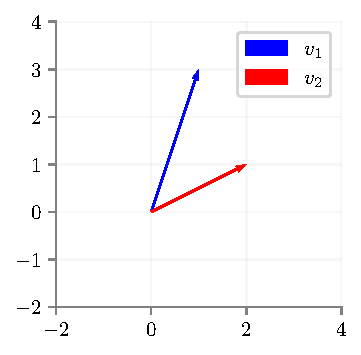
\includegraphics{../assets/linear-regression/figures/geoemetric-span-1.pdf}



\end{frame}

\begin{frame}{Example}

    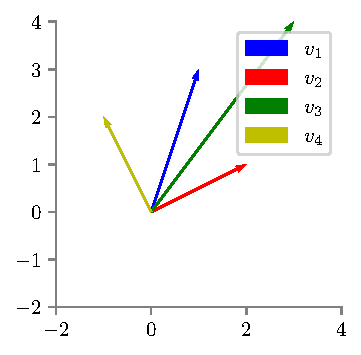
\includegraphics{../assets/linear-regression/figures/geoemetric-span-2.pdf}

    We have $v_3 = v_1 + v_2$ \\
    We have $v_4 = v_1 - v_2$ \\


\end{frame}

\begin{frame}{Example}
    Simulating the above example in python using different values of $\alpha_1$ and $\alpha_2$


    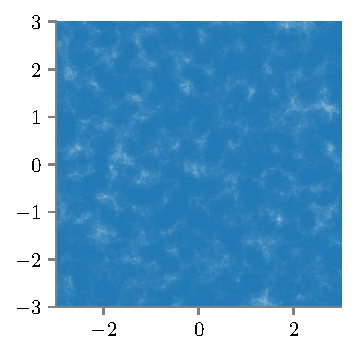
\includegraphics{../assets/linear-regression/figures/geoemetric-span-3.pdf}
    
    Span(($v_1, v_2$)) $\in \mathcal{R}^2$
\end{frame}


\begin{frame}{Example}
Find the span of ($\begin{bmatrix}
1 \\2
\end{bmatrix}, \begin{bmatrix}
2 \\4
\end{bmatrix}) $

\pause Can we obtain a point (x, y) s.t. x = 3y? \\
\pause No \\ 
\pause Span of the above set is along the line y = 2x

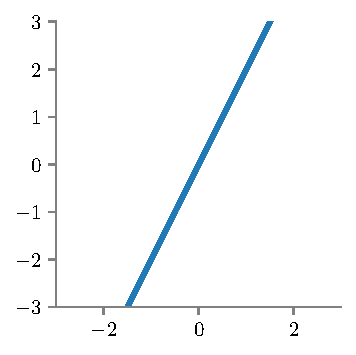
\includegraphics[scale=0.6]{../assets/linear-regression/figures/geoemetric-span-4.pdf}


\end{frame}

\begin{frame}{Example}
Find the span of ($\begin{bmatrix}
1 \\1\\1
\end{bmatrix}, \begin{bmatrix}
2 \\-2\\2
\end{bmatrix}) $
\pause 
    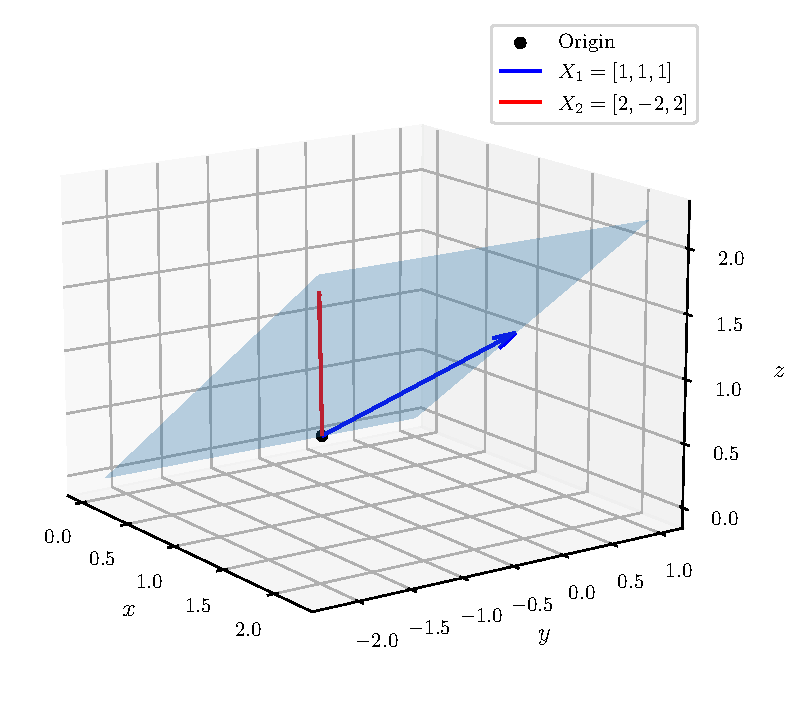
\includegraphics[width=0.6\textwidth]{../assets/linear-regression/figures/geometric-1.pdf}


\pause The span is the plane $z=x$ or $x_3=x_1$
\end{frame}

\begin{frame}{Geometric Interpretation}
Consider $\mX$ and $\vy$ as follows. 
$$
\mX=\left(\begin{array}{cc}
{1} & {2} \\
{1} & {-2} \\
{1} & {2}
\end{array}\right), \quad \vy=\left(\begin{array}{c}
{8.8957} \\
{0.6130} \\
{1.7761}
\end{array}\right)
$$
\begin{itemize}[<+->]
\item We are trying to learn $\vtheta$ for $\yhat=\mX\vtheta$ such that $\vert \vert \vy - \yhat \vert \vert_{2}$ is minimised
\item Consider the two columns of $\mX$. Can we write $\mX\vtheta$ as the span of ($\begin{bmatrix}
1 \\1\\1
\end{bmatrix}, \begin{bmatrix}
2 \\-2\\2
\end{bmatrix}$)?
\item We wish to find $\yhat$ such that 
$$
\underset{\yhat \in SPAN\{\bar{x_{1}},\bar{x_{2}},\dots,\bar{x_{D}}\} } \argmin \vert \vert \vy - \yhat \vert \vert_{2}
$$
\end{itemize}

\end{frame}


\begin{frame}{Geometric Interpretation}
Span of ($\begin{bmatrix}
1 \\1\\1
\end{bmatrix}, \begin{bmatrix}
2 \\-2\\2
\end{bmatrix}) $


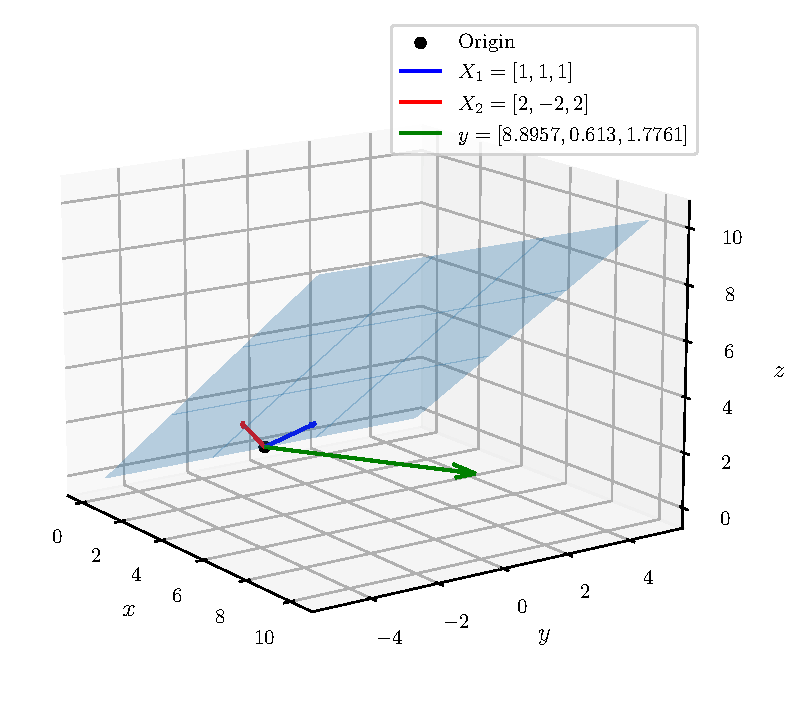
\includegraphics[width=0.6\textwidth]{../assets/linear-regression/figures/geometric-2.pdf}

\end{frame}


\begin{frame}{Geometric Interpretation}	

    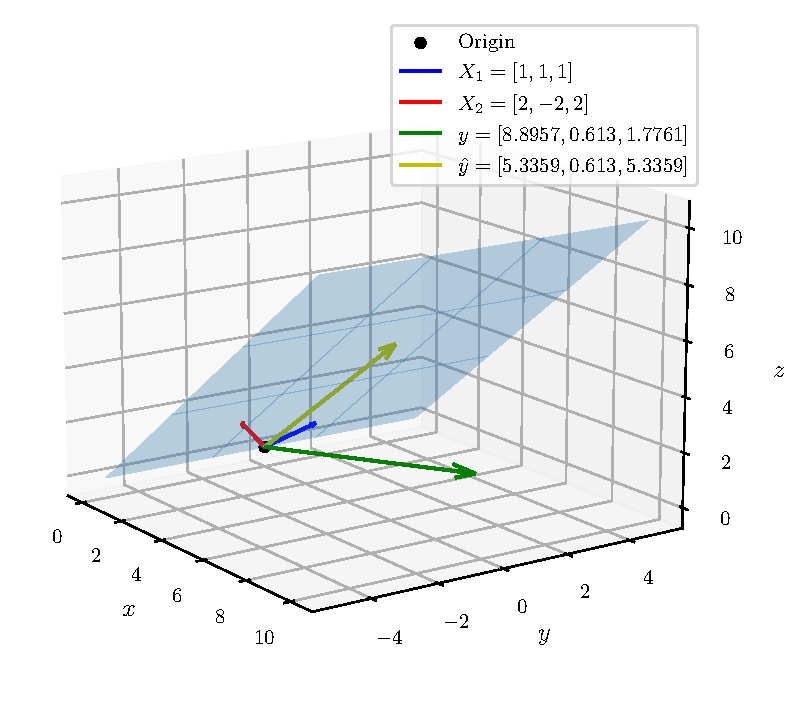
\includegraphics[width=0.6\textwidth]{../assets/linear-regression/figures/geometric-3.pdf}

    


\begin{itemize}[<+->]
\item We seek a $\hat{y}$ in the span of the columns of $X$ such that it is closest to $y$
\end{itemize}

\end{frame}


\begin{frame}{Geometric Interpretation}	

    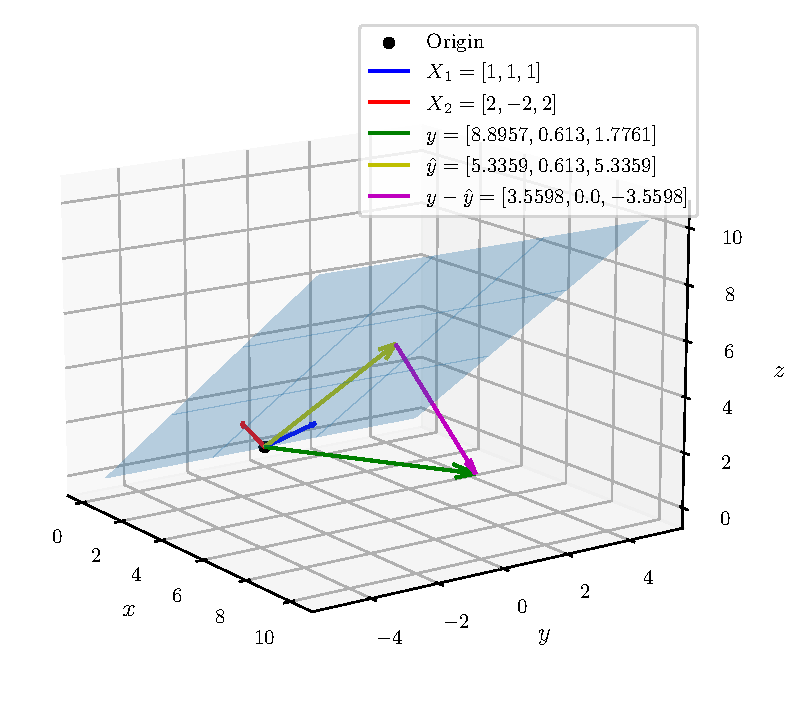
\includegraphics[width=0.6\textwidth]{../assets/linear-regression/figures/geometric-4.pdf}

    


\begin{itemize}[<+->]
\item This happens when $y-\hat{y}\perp x_j \forall j$ or $x_j^T(y-\hat{y})=0$
\item $X^T(y-X\theta)=0$
\item $X^Ty = X^TX\theta$ or $\hat{\theta} =(X^TX)^{-1}X^Ty$ 
\end{itemize}

\end{frame}

\section{Dummy Variables and Multicollinearity}
\begin{frame}{Multi-collinearity}
    There can be situations where inverse of $X^{T}X$ is not computable. \\
    \pause This condition arises when the $|X^{T}X|$ = 0.
    
    \begin{equation}
    X = \begin{bmatrix}
    1 & 1& 2\\
    1 & 2& 4\\
    1 & 3& 6\\
    \end{bmatrix}
    \end{equation}
    
    \pause The matrix X is not full rank. 
    \end{frame}
    
    
    
    
    
    \begin{frame}{Multi-collinearity}
    
    It arises when one or more predictor variables/features in X can be expressed as a linear combination of others\\
    \vspace{5mm}
    
    
    
    How to tackle it?
    \begin{itemize}
        \item<+-> Regularize
        \item<+-> Drop variables
        \item<+-> Avoid dummy variable trap
    \end{itemize}
    \end{frame}
    \begin{frame}{Dummy variables}
    Say Pollution in Delhi = P
    \pause \begin{center}
        P = $\theta_{0}$ + $\theta_{1}$*\#Vehicles + $\theta_{1}$*
        \textit{Wind speed} + $\theta_{3}$ * \textit{Wind Direction}
    \end{center}
    
    \pause But, wind direction is a categorical variable. \\
    \pause It is denoted as follows \{N:0, E:1, W:2, S:3 \}\\
    \vspace{3em}
    
    \pause Can we use the direct encoding? \\
    \pause Then this implies that S$>$W$>$E$>$N
    \end{frame}
    
    \begin{frame}{Dummy Variables}
    \begin{center}
    
    N-1 Variable encoding\\
    \vspace{1em}
    \begin{tabular}{|c|c|c|c|}
        \hline
        & Is it N? &Is it E? &Is it W?\\
        \hline
        \hline
        N & 1&0&0 \\
        E & 0&1&0\\
        W & 0&0&1\\
        S & 0&0&0\\
        \hline
    \end{tabular}
    
    \end{center}
    \end{frame}
    
    
    \begin{frame}{Dummy Variables}
    \begin{center}
    
    N Variable encoding\\
    \vspace{1em}
    \begin{tabular}{|c|c|c|c|c|}
    \hline
    & Is it N? &Is it E? &Is it W? & Is it S?\\
    \hline
    \hline
    N & 1&0&0&0 \\
    E & 0&1&0&0\\
    W & 0&0&1&0\\
    S & 0&0&0&1\\
    \hline
    \end{tabular}
    \end{center}
    \end{frame}
    
    
    
    \begin{frame}{Dummy Variables}
    Which is better N variable encoding or N-1 variable encoding? \\
    
    \pause The N-1 variable encoding is better because the N variable encoding can cause multi-collinearity. \\
    
    \pause Is it S = 1 - (Is it N + Is it W + Is it E) 
    
    \end{frame}
    
    
    \begin{frame}{Binary Encoding}
    
    \begin{center}
    \begin{tabular}{|c|c|}
    \hline
    N & 00 \\
    E& 01\\
    W & 10\\
    S& 11\\
    \hline
    \end{tabular}\\
    \end{center}
    
    
    \vspace{1em}
    \pause W and S are related by one bit. 
    
    \pause This introduces dependencies between them, and this can cause confusion in classifiers.
    \end{frame}
    
    \begin{frame}{Interpreting Dummy variables}
    \begin{center}
    \begin{tabular}{c|c}
    Gender& height\\
    \hline
    \hline
    F & \dots \\
    F & \dots \\
    F & \dots \\
    M & \dots \\
    M & \dots \\
    \end{tabular}
    
    \end{center}
    
    \pause Encoding
    
    \begin{center}
    \pause \begin{tabular}{c|c}
    Is Female& height\\
    \hline
    \hline
    1 & \dots \\
    1 & \dots \\
    1 & \dots \\
    0 & \dots \\
    0 & \dots \\
    \end{tabular}
    \end{center}
    
    \end{frame}
    
    \begin{frame}{Interpreting Dummy Variables}
    \begin{center}
        \pause \begin{tabular}{c|c}
            Is Female& height\\
            \hline
            \hline
            1 & 5 \\
            1 & 5.2 \\
            1 & 5.4 \\
            0 & 5.8 \\
            0 & 6 \\
        \end{tabular}
    \end{center}
    \pause $height_{i}$ = $\theta_{0}$ + $\theta_{1}$ *  (Is Female) + $\epsilon_{i}$\\
    \vspace{1em}
    \pause We get $\theta_0$ = 5.9 and $\theta_1$ = -0.7\\
    \pause $\theta_{0}$ = Avg height of Male = 5.9\\
    \pause $\theta_{0} + \theta_{1}$ is chosen based (equal to) on 5, 5.2, 5.4 (for three records). \\
    \pause $\theta_{1}$ is chosen based on 5-5.9, 5.2-5.9, 5.4-5.9
    \pause $\theta_{1}$ = Avg. female height (5+5.2+5.4)/3 - Avg. male height(5.9)
    \end{frame}
    
    \begin{frame}{Interpreting Dummy Variables}
    Alternatively, instead of a 0/1 coding scheme, we could create a dummy variable
    
    \pause \(x_{i}=\left\{\begin{array}{ll}{1} & {\text { if } i \text { th person is female }} \\ {-1} & {\text { if } i \text { th person is male }}\end{array}\right.\)
    
    \pause \(y_{i}=\theta_{0}+\theta_{1} x_{i}+\epsilon_{i}=\left\{\begin{array}{ll}{\theta_{0}+\theta_{1}+\epsilon_{i}} & {\text { if } i \text { th person is female }} \\ {\theta_{0}-\theta_{1}+\epsilon_{i}} & {\text { if } i \text { th person is male. }}\end{array}\right.\)
    
    
    \pause Now, $\theta_{0}$ can be interpreted as average person height. $\theta_{1}$ as the amount that female height is above average and male height is below average.
    \end{frame}



\end{document}
